% DO NOT COMPILE THIS FILE DIRECTLY!
% This is included by the other .tex files.

\begin{frame}
\titlepage
\end{frame}

\begin{frame}
  \frametitle{What changed since the last workshop?}
  \begin{itemize}
    \item ATT\&CK has been steadily on the rise
    \item In cyber security MISP information sharing community, ATT\&CK is often attached on {\bf more than 70\%} of the events
    \item The {\bf number of matrix-like galaxies increased} in MISP in addition to the ones published by MITRE
        \begin{itemize}
                \item Including {\bf Telecom} matrix (Bhadra framework), {\bf Election guidelines}, {\bf Misinformation patterns}, {\bf Segregation of Duties (LEA/CSIRT)}, {\bf Financial} (att4ck for fraud), {\bf Office 365} techniques.
        \end{itemize}
  \end{itemize}
\end{frame}

\begin{frame}
  \frametitle{MISP updates about ATT\&CK}
  \begin{itemize}
    \item Various improvements in ATT\&CK visualisations and export format such as {\bf attack-sightings}
    \item {\bf ATT\&CK Sub-techniques} are now available MISP
    \item MITRE ATT\&CK {\bf ICS} is available
    \item Challenges with historical data and ATT\&CK techniques. Should MITRE provide UUID mapping tables for new and old/historical techniques?
  \end{itemize}
\end{frame}

\begin{frame}
  \frametitle{MISP event report}
  \begin{itemize}
        \item Event report\footnote{\url{https://www.misp-project.org/2020/10/16/MISP.2.4.133.released.html}} is a new convenient mechanism to edit, visualize and share Markdown reports in MISP
        \item Standardise and {\bf extend the Markdown format} to support references to MISP attributes, objects, galaxies or ATT\&CK matrix:
  \end{itemize}
        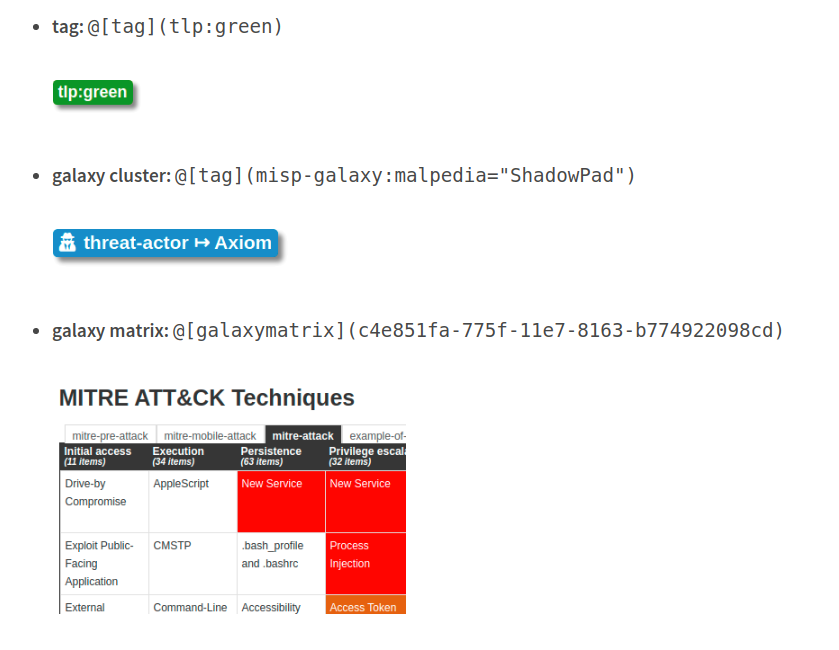
\includegraphics[scale=0.2]{report.png}
\end{frame}

\begin{frame}
  \frametitle{MISP event report}
  \begin{itemize}
        \item Overall goal is to provide a standard Markdown format for reports which can be combined with structured elements
        \item The importance of {\bf fixed references in MITRE ATT\&CK is critical} for long-term accessibility to information
        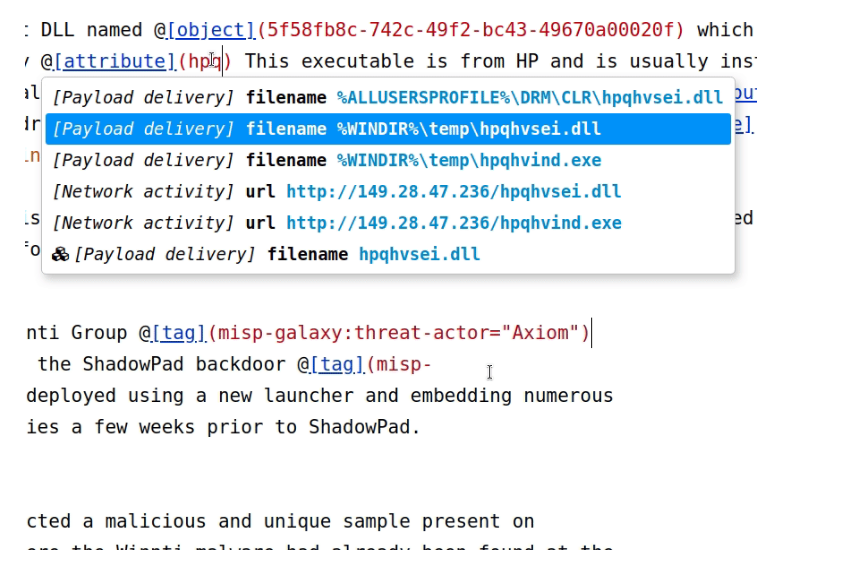
\includegraphics[scale=0.25]{view.png}
  \end{itemize}

\end{frame}


\begin{frame}
        \frametitle{Conclusion}
        \begin{itemize}
                \item Bridging the gap between structured and unstructured report is critical. Integrating tram\footnote{\url{https://github.com/mitre-attack/tram}} with MISP event report could be an option.
                \item The matrix-like enhancement from the MISP galaxy format will be added in the default MISP galaxy standard format\footnote{\url{https://www.misp-standard.org/}}
                \item ATT\&CK like matrices become more and more common and used, thanks the {\bf continuous work of the community}
        \end{itemize}
\end{frame}

